\documentclass[a4paper]{article}

% --- UNIVERSAL PREAMBLE BLOCK ---
\usepackage[a4paper, top=1.5cm, bottom=1.5cm, left=1.5cm, right=1.5cm]{geometry}
\usepackage{fontspec}

\usepackage[indonesian, provide=*]{babel}
\babelprovide[import, onchar=ids fonts]{indonesian}
\babelprovide[import, onchar=ids fonts]{english}

% Set default/Latin font to Sans Serif (Noto Sans)
\babelfont{rm}{Noto Sans}
\babelfont{sf}{Noto Sans}

% Packages for graphics and layout
\usepackage{tikz}
\usetikzlibrary{shapes, shapes.symbols, arrows.meta, positioning, calc, shadows, backgrounds, patterns, decorations.pathreplacing, 3d}
\usepackage[most]{tcolorbox}
\usepackage{multicol}
\usepackage{enumitem}

% --- COLOR DEFINITIONS ---
\definecolor{mainBlue}{HTML}{2C3E50}
\definecolor{accentTeal}{HTML}{16A085}
\definecolor{alertRed}{HTML}{E74C3C}
\definecolor{niceOrange}{HTML}{F39C12}
\definecolor{powerBlue}{HTML}{2980B9}
\definecolor{cubeRed}{HTML}{C0392B}
\definecolor{softBgA}{HTML}{ECF0F1}
\definecolor{softBgB}{HTML}{F7F9F9}
\definecolor{solGreen}{HTML}{27AE60}
\definecolor{lightPurple}{HTML}{9B59B6}

% --- DRAWING SETTINGS ---
% Depth settings for 3D effect (Oblique Projection)
\def\xslant{0.3}
\def\yslant{0.2}

% --- IMPROVED DIENES COMMANDS (CONSISTENT 3D) ---

% 1. Unit (Satuan) - Small Cube
\newcommand{\DrawUnit}[2]{
    \begin{scope}[shift={(#1,#2)}]
        % Front face
        \draw[fill=niceOrange!80, draw=mainBlue, thick] (0,0) rectangle (0.5,0.5);
        % Top face
        \draw[fill=niceOrange!60, draw=mainBlue, thick] (0,0.5) -- (\xslant, 0.5+\yslant) -- (0.5+\xslant, 0.5+\yslant) -- (0.5, 0.5) -- cycle;
        % Side face
        \draw[fill=niceOrange!40, draw=mainBlue, thick] (0.5,0) -- (0.5+\xslant, \yslant) -- (0.5+\xslant, 0.5+\yslant) -- (0.5, 0.5) -- cycle;
    \end{scope}
}

% 2. Long (Puluhan) - Tall Prism with markings
\newcommand{\DrawLong}[2]{
    \begin{scope}[shift={(#1,#2)}]
        % Front face
        \draw[fill=accentTeal!80, draw=mainBlue, thick] (0,0) rectangle (0.5, 5);
        % Top face
        \draw[fill=accentTeal!60, draw=mainBlue, thick] (0,5) -- (\xslant, 5+\yslant) -- (0.5+\xslant, 5+\yslant) -- (0.5, 5) -- cycle;
        % Side face
        \draw[fill=accentTeal!40, draw=mainBlue, thick] (0.5,0) -- (0.5+\xslant, \yslant) -- (0.5+\xslant, 5+\yslant) -- (0.5, 5) -- cycle;
        % Lines for units
        \foreach \y in {0.5, 1.0, ..., 4.5} {
            \draw[mainBlue, thin] (0,\y) -- (0.5,\y); % Front lines
            \draw[mainBlue, thin] (0.5,\y) -- (0.5+\xslant, \y+\yslant); % Side lines
        }
    \end{scope}
}

% 3. Flat (Ratusan) - Flat Prism with grid
\newcommand{\DrawFlat}[2]{
    \begin{scope}[shift={(#1,#2)}]
        % Front face
        \draw[fill=powerBlue!60, draw=mainBlue, thick] (0,0) rectangle (5, 5);
        % Top face
        \draw[fill=powerBlue!40, draw=mainBlue, thick] (0,5) -- (\xslant, 5+\yslant) -- (5+\xslant, 5+\yslant) -- (5, 5) -- cycle;
        % Side face
        \draw[fill=powerBlue!30, draw=mainBlue, thick] (5,0) -- (5+\xslant, \yslant) -- (5+\xslant, 5+\yslant) -- (5, 5) -- cycle;
        % Grid Lines
        \draw[mainBlue, thin, step=0.5] (0,0) grid (5,5);
    \end{scope}
}

% 4. Thousand (Ribuan) - Large Cube
\newcommand{\DrawThousand}[2]{
    \begin{scope}[shift={(#1,#2)}]
        \def\bigdX{2.5} % Scaled depth X
        \def\bigdY{1.5} % Scaled depth Y
        
        % Front face
        \draw[fill=cubeRed!60, draw=mainBlue, thick] (0,0) rectangle (5,5);
        \draw[mainBlue, thin, step=0.5] (0,0) grid (5,5);
        
        % Top face
        \draw[fill=cubeRed!40, draw=mainBlue, thick] (0,5) -- (\bigdX, 5+\bigdY) -- (5+\bigdX, 5+\bigdY) -- (5,5) -- cycle;
        % Side face
        \draw[fill=cubeRed!80, draw=mainBlue, thick] (5,0) -- (5+\bigdX, \bigdY) -- (5+\bigdX, 5+\bigdY) -- (5,5) -- cycle;
        
        % Grid lines on top/side for realistic look
        \foreach \k in {0, 0.5, ..., 5} {
             \draw[mainBlue, very thin] (\k, 5) -- (\k + \bigdX, 5 + \bigdY); % Top vertical
             \draw[mainBlue, very thin] (5, \k) -- (5 + \bigdX, \k + \bigdY); % Side horizontal
        }
    \end{scope}
}

\newcommand{\checkbox}{\tikz[baseline=-0.6ex]{\draw[thick, mainBlue] (0,0) rectangle (0.3,0.3);}}

% --- CUSTOM BOX FOR CASE STUDIES ---
\newtcolorbox{CaseStudyBox}[2][]{
    enhanced,
    colback=white,
    colframe=mainBlue!20!white,
    boxrule=0.5pt,
    left=2mm, right=2mm, top=2mm, bottom=2mm,
    title={\textbf{#2}},
    coltitle=mainBlue,
    fonttitle=\bfseries\large,
    attach boxed title to top left={yshift=-2mm, xshift=2mm},
    boxed title style={boxrule=0pt, colframe=white, colback=white},
    #1
}

\begin{document}

% =================================================================================
% PART 1: INTRODUCTION & CONTEXT (RESTORED)
% =================================================================================

\tikzset{
    blockPic/.style={scale=0.5, baseline={([yshift=-.5ex]current bounding box.center)}},
    arrowFlow/.style={->, >={Latex[width=3mm,length=3mm]}, ultra thick, draw=accentTeal},
    conceptBox/.style={
        rectangle, rounded corners, draw=none, fill=white, drop shadow,
        text width=4.5cm, align=center, minimum height=2cm, font=\small
    }
}

% --- HEADER PART 1 ---
\begin{tcolorbox}[colback=mainBlue, colframe=mainBlue, arc=0mm, boxrule=0pt, top=5mm, bottom=5mm, halign=center]
    {\Huge \bfseries \color{white} BLOK DIENES (BASE TEN BLOCKS)} \\
    \vspace{0.2cm}
    {\large \color{accentTeal} \textbf{Visualisasi Konkret Nilai Tempat \& Algoritma}}
\end{tcolorbox}

\vspace{0.2cm}

% --- SECTION 1: KONTEKS MASALAH & SOLUSI ---
\begin{tcolorbox}[title=\textbf{1. KONTEKS: MENGAPA KITA BUTUH ALAT INI?}, colback=white, colframe=lightPurple, coltitle=white, fonttitle=\bfseries\large]
    \begin{minipage}[t]{0.48\textwidth}
        \textcolor{alertRed}{\Large \textbf{A. Masalah: "Abstract Symbols"}}
        \vspace{0.1cm}
        \begin{itemize}[leftmargin=*, itemsep=2pt]
            \item \textbf{Kebingungan Posisi:} Siswa melihat "2" pada angka "24" sama besarnya dengan "2" pada angka "2".
            \item \textbf{Tanpa Proporsi:} Simbol angka tidak menunjukkan ukuran (magnitude).
        \end{itemize}
    \end{minipage}%
    \hfill
    \begin{minipage}[t]{0.48\textwidth}
        \textcolor{accentTeal}{\Large \textbf{B. Solusi: Blok Dienes}}
        \vspace{0.1cm}
        \begin{itemize}[leftmargin=*, itemsep=2pt]
            \item \textbf{Proporsional:} Blok puluhan secara fisik \textbf{10x lebih besar} dari satuan.
            \item \textbf{Visualisasi Grup:} Memperjelas konsep "Satu Puluhan" adalah kumpulan "Sepuluh Satuan".
        \end{itemize}
    \end{minipage}
\end{tcolorbox}

% --- SECTION 2: ANATOMI & KONSISTENSI UKURAN ---
\begin{tcolorbox}[title=\textbf{2. ANATOMI: KONSISTENSI VISUAL 3D}, colback=white, colframe=accentTeal, coltitle=white, fonttitle=\bfseries\large]
    \centering
    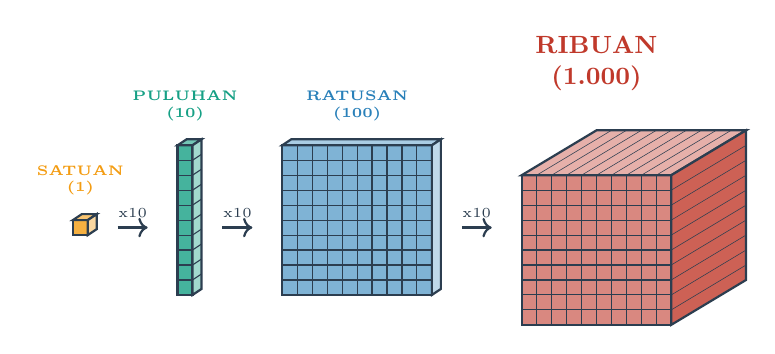
\begin{tikzpicture}[scale=0.38, baseline={([yshift=-.5ex]current bounding box.center)}]
        % Unit
        \DrawUnit{0}{3} 
        \node[above, font=\bfseries\tiny, text=niceOrange, align=center] at (0.25, 4) {SATUAN\\(1)};
        
        \draw[->, mainBlue, thick] (1.5, 3.25) -- (2.5, 3.25) node[midway, above, font=\tiny] {x10};
        
        % Long
        \DrawLong{3.5}{1} 
        \node[above, font=\bfseries\tiny, text=accentTeal, align=center] at (3.75, 6.5) {PULUHAN\\(10)};
        
        \draw[->, mainBlue, thick] (5, 3.25) -- (6, 3.25) node[midway, above, font=\tiny] {x10};
        
        % Flat
        \DrawFlat{7}{1} 
        \node[above, font=\bfseries\tiny, text=powerBlue, align=center] at (9.5, 6.5) {RATUSAN\\(100)};
        
        \draw[->, mainBlue, thick] (13, 3.25) -- (14, 3.25) node[midway, above, font=\tiny] {x10};
        
        % Cube
        \DrawThousand{15}{0} 
        \node[above, font=\bfseries\small, text=cubeRed, align=center] at (17.5, 7.5) {RIBUAN\\(1.000)};
    \end{tikzpicture}
    \vspace{0.2cm} \hrule \vspace{0.2cm}
    \begin{minipage}{0.9\textwidth}
        \textbf{Prinsip "Trading" (Tukar) Bertingkat:}
        \begin{itemize}[leftmargin=*, label=\checkbox]
            \item \textbf{10 Unit} $\rightarrow$ Tukar jadi \textbf{1 Long}.
            \item \textbf{10 Long} $\rightarrow$ Tukar jadi \textbf{1 Flat}.
            \item \textbf{10 Flat} $\rightarrow$ Tukar jadi \textbf{1 Cube}.
        \end{itemize}
    \end{minipage}
\end{tcolorbox}

% --- SECTION 3: JEMBATAN C-P-A ---
\begin{tcolorbox}[title=\textbf{3. JEMBATAN C-P-A (TRANSISI KE ABSTRAK)}, colback=softBgA, colframe=niceOrange, coltitle=white, fonttitle=\bfseries\large]
    \centering
    \begin{tikzpicture}[node distance=0.2cm and 0.5cm]
        \node[conceptBox] (concrete) {
            \textbf{A. KONKRET}\\ \textit{"Pegang Bloknya"}\\ \vspace{0.1cm}
            \begin{tikzpicture}[scale=0.2] \DrawLong{0}{0} \DrawUnit{1}{0} \DrawUnit{1}{0.7} \end{tikzpicture}
        };
        \node[conceptBox, right=of concrete] (bridge) {
            \textbf{B. PIKTORIAL}\\ \textit{"Gambar Sketsa"}\\ \vspace{0.1cm}
            
\begin{tikzpicture}[scale=0.25] \draw[thick, mainBlue] (0,0) -- (0,5); \fill[mainBlue] (1,0.5) circle (0.2); \fill[mainBlue] (1.5,0.5) circle (0.2); \end{tikzpicture}
        };
        \node[conceptBox, right=of bridge] (pictorial) {
            \textbf{C. ABSTRAK}\\ \textit{"Simbol Angka"}\\ \vspace{0.1cm}
            \tikz{\node[cloud, cloud puffs=8, draw, fill=gray!10, font=\bfseries\Large] {12};}
        };
        \draw[arrowFlow] (concrete) -- (bridge); \draw[arrowFlow] (bridge) -- (pictorial);
    \end{tikzpicture}
\end{tcolorbox}

\newpage

% =================================================================================
% PART 2: MASTERY CASE STUDIES
% =================================================================================

\tikzset{
    blockPic/.style={scale=0.4, baseline={([yshift=-.5ex]current bounding box.center)}},
    crossOut/.style={cross out, draw=alertRed, very thick, minimum size=0.6cm},
    arrowOp/.style={->, >={Latex}, thick, dashed, color=alertRed}
}

% --- HEADER PART 2 ---
\begin{tcolorbox}[colback=mainBlue, colframe=mainBlue, arc=0mm, boxrule=0pt, top=4mm, bottom=4mm, halign=center]
    {\Huge \bfseries \color{white} DIENES MASTERY} \\
    \vspace{0.1cm}
    {\large \color{accentTeal} \textbf{Bedah Konsep Operasi Bilangan}}
\end{tcolorbox}
\vspace{0.3cm}

% --- KASUS 1 ---
\begin{CaseStudyBox}{KASUS 1: MAGNITUDE "24 vs 42"}
\begin{minipage}{0.4\textwidth}
    \centering
    \begin{tikzpicture}[blockPic, scale=0.8]
        % 24 Area
        \node[font=\bfseries, mainBlue] at (1, 6.5) {24};
        \DrawLong{0}{0} \DrawLong{0.8}{0}
        \foreach \y in {0,1,2,3} \DrawUnit{2}{\y*0.8};
        
        % Separator
        \draw[dashed, mainBlue!30] (3.5, -1) -- (3.5, 7);

        % 42 Area
        \node[font=\bfseries, mainBlue] at (6, 6.5) {42};
        \DrawLong{4}{0} \DrawLong{4.8}{0} \DrawLong{5.6}{0} \DrawLong{6.4}{0}
        \foreach \y in {0,1} \DrawUnit{7.5}{\y*0.8};
        
        % Visual Cue
        \draw[decorate, decoration={brace, mirror, amplitude=5pt}, thick, alertRed] (4, -0.5) -- (7.2, -0.5) node[midway, below=5pt, font=\tiny] {LEBIH BANYAK!};
    \end{tikzpicture}
\end{minipage}%
\hfill
\begin{minipage}{0.58\textwidth}
    \textbf{Visualisasi:} Dengan memberikan efek 3D, siswa melihat bahwa 4 batang puluhan pada "42" secara fisik menempati ruang (volume) yang jauh lebih besar daripada 2 batang puluhan pada "24".
\end{minipage}
\end{CaseStudyBox}

\vspace{0.3cm}

% --- KASUS 2 ---
\begin{CaseStudyBox}{KASUS 2: PENJUMLAHAN MENYIMPAN ($18 + 5$)}
\begin{minipage}{0.45\textwidth}
    \centering
    \begin{tikzpicture}[blockPic, scale=0.8] 
        % Context - Moved Higher to y=7.5
        \node[font=\bfseries\tiny, anchor=west, align=left] at (0, 7.5) {Awal:\\8 Satuan + 5 Satuan};
        \DrawLong{0}{0} 
        
        % 8 units
        \foreach \y in {0,...,3} \DrawUnit{1.5}{\y*0.7};
        \foreach \y in {0,...,3} \DrawUnit{2.2}{\y*0.7};
        
        % 5 units (additions)
        \foreach \y in {0,...,4} \DrawUnit{3.5}{\y*0.7};
        
        % Grouping Ring (Circle 10 units)
        \draw[alertRed, thick, rounded corners] (1.3, -0.2) rectangle (3.0, 3.0); 
        \draw[alertRed, thick, rounded corners] (3.3, -0.2) rectangle (4.2, 1.0); 
        \draw[alertRed, thick] (3.0, 0.5) -- (3.3, 0.5); 
        
        % Label moved to (3.5, 5.5) with white background to prevent clutter
        \node[font=\bfseries\tiny, text=alertRed, fill=white, inner sep=1pt] at (3.5, 5.5) {JADI 1 PULUHAN};
        
        % Arrow start from grouping box top (y=3.5) to destination
        \draw[arrowOp, ultra thick] (3, 3.5) to[out=60, in=150] (6.0, 5.5);
        
        % Result - Moved Higher to y=7.5
        \node[font=\bfseries\tiny, anchor=west] at (6.0, 7.5) {Hasil: 23};
        \DrawLong{6.0}{0} \DrawLong{6.8}{0} % 2 Tens
        \foreach \y in {2,3,4} \DrawUnit{8.5}{\y*0.7 - 1.4}; % 3 remaining units
    \end{tikzpicture}
\end{minipage}%
\hfill
\begin{minipage}{0.52\textwidth}
    \textbf{Konsep:} "Bundling". Ketika satuan menumpuk lebih dari 9, visualisasikan ikatan merah yang menyatukan 10 satuan menjadi 1 batang utuh baru.
\end{minipage}
\end{CaseStudyBox}

\vspace{0.3cm}

% --- KASUS 3 ---
\begin{CaseStudyBox}{KASUS 3: PENGURANGAN MEMINJAM ($32 - 15$)}
\begin{minipage}{0.45\textwidth}
    \centering
    \begin{tikzpicture}[scale=0.35, baseline={([yshift=-.5ex]current bounding box.center)}]
        \node[font=\bfseries\tiny, mainBlue] at (2, 6) {Pecah Puluhan};
        % 3 Tens initially
        \DrawLong{0}{0} \DrawLong{1}{0} 
        % Exploded Ten
        \node[crossOut] at (2.25, 2.5) {}; 
        \DrawLong{2}{0}
        
        \draw[arrowOp] (2.5, 2.5) -- (4.5, 2.5);
        
        % The exploded units
        \foreach \y in {0,1} \foreach \x in {5,6,7,8,9} \DrawUnit{\x}{\y};
        
        % The original 2 units
        \DrawUnit{10}{0} \DrawUnit{10}{1}
        
        % Subtract 5 (Cross out)
        \foreach \x in {5,6,7,8,9} \node[crossOut] at (\x.25, 0.25) {};
        \node[font=\tiny, text=alertRed] at (7.5, -1.5) {Buang 5};
        
        % Brace showing result
        \draw[decorate, decoration={brace, amplitude=3pt}, thick, solGreen] (5, 1.8) -- (10.5, 1.8) node[midway, above=2pt, font=\tiny] {Sisa 7};
    \end{tikzpicture}
\end{minipage}%
\hfill
\begin{minipage}{0.52\textwidth}
    \textbf{Konsep:} "Unbundling/Decompose". Jangan gunakan istilah "pinjam" (karena tidak dikembalikan), gunakan "Tukar" atau "Pecah". Visualisasikan 1 batang hancur menjadi 10 keping.
\end{minipage}
\end{CaseStudyBox}

\vspace{0.3cm}

% --- KASUS 4 ---
\begin{CaseStudyBox}{KASUS 4: PERKALIAN AREA DISTRIBUTIF ($12 \times 3$)}
\begin{minipage}{0.45\textwidth}
    \centering
    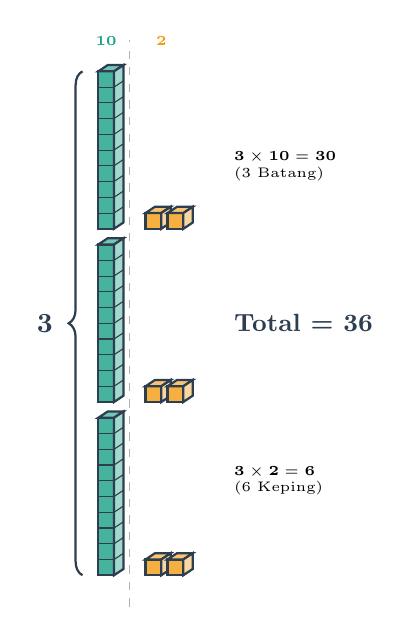
\begin{tikzpicture}[scale=0.4, baseline={([yshift=-.5ex]current bounding box.center)}]
        % Row 1
        \DrawLong{0}{0} \DrawUnit{1.5}{0} \DrawUnit{2.2}{0}
        % Row 2
        \DrawLong{0}{5.5} \DrawUnit{1.5}{5.5} \DrawUnit{2.2}{5.5}
        % Row 3
        \DrawLong{0}{11} \DrawUnit{1.5}{11} \DrawUnit{2.2}{11}

        % Grouping Braces
        \draw[decorate, decoration={brace, amplitude=5pt}, thick, mainBlue] (-0.5, 0) -- (-0.5, 16) node[midway, left=7pt, font=\bfseries] {3};
        
        % Top Labels showing distribution
        \node[above, font=\bfseries\tiny, text=accentTeal] at (0.25, 16.5) {10};
        \node[above, font=\bfseries\tiny, text=niceOrange] at (2, 16.5) {2};
        
        % Calculation
        \node[right, align=left, font=\tiny] at (4, 13) {$\mathbf{3 \times 10 = 30}$\\(3 Batang)};
        \node[right, align=left, font=\tiny] at (4, 3) {$\mathbf{3 \times 2 = 6}$\\(6 Keping)};
        \node[right, font=\bfseries\small, mainBlue] at (4, 8) {Total = 36};
        
        % Separation Line
        \draw[dashed, mainBlue!40] (1.0, -1) -- (1.0, 17);
    \end{tikzpicture}
\end{minipage}%
\hfill
\begin{minipage}{0.52\textwidth}
    \textbf{Konsep:} "Area Model". Pisahkan secara visual kolom puluhan dan kolom satuan. Ini membangun pondasi mental untuk aljabar $(x + 2)$ dan perkalian bersusun ke bawah.
\end{minipage}
\end{CaseStudyBox}

\vspace{0.3cm}

% --- KASUS 5 ---
\begin{CaseStudyBox}{KASUS 5: PEMBAGIAN PARTISI ($42 \div 3$)}
\begin{minipage}{0.45\textwidth}
    \centering
    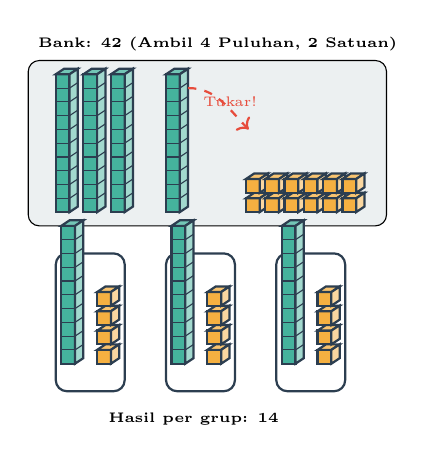
\begin{tikzpicture}[scale=0.35, baseline={([yshift=-.5ex]current bounding box.center)}]
        % --- BANK UTAMA ---
        % Enlarge the bank box to avoid crowding
        \draw[fill=softBgA, rounded corners] (-1, 5) rectangle (12, 11);
        \node[anchor=south west, font=\tiny\bfseries] at (-1, 11) {Bank: 42 (Ambil 4 Puluhan, 2 Satuan)};
        
        % 3 Tens easy distribute
        \DrawLong{0}{5.5} \DrawLong{1}{5.5} \DrawLong{2}{5.5}
        
        % The Remainder Ten (At x=4)
        \DrawLong{4}{5.5}
        
        % Arrow moved to avoid text overlap
        \draw[->, thick, alertRed, dashed] (4.8, 10) to[out=0, in=135] (7, 8.5);
        
        % Text moved to the RIGHT of the block (x=5.0)
        \node[font=\tiny, text=alertRed, anchor=west] at (5.0, 9.5) {Tukar!};
        
        % Converted Units
        \foreach \y in {0,1} \foreach \x in {7,8,9,10,11,12} \DrawUnit{\x*0.7 + 2}{\y*0.7 + 5.5};
        
        % --- GROUPING BOXES ---
        \foreach \gx/\lbl in {0/A, 4/B, 8/C} {
            \draw[mainBlue, thick, rounded corners] (\gx, -1) rectangle (\gx+2.5, 4);
            % Distributed Ten
            \DrawLong{\gx+0.2}{0}
            % Distributed Units (4 per box)
            \foreach \uy in {0,1,2,3} \DrawUnit{\gx+1.5}{\uy*0.7};
        }
        \node[font=\bfseries\tiny] at (5, -2) {Hasil per grup: 14};

    \end{tikzpicture}
\end{minipage}%
\hfill
\begin{minipage}{0.52\textwidth}
    \textbf{Konsep:} "Partisi Adil".
    1. Bagi puluhan yang utuh dulu (3 batang ke 3 kotak).
    2. Sisa 1 batang tidak bisa dibagi $\rightarrow$ Tukar jadi 10 keping.
    3. Gabung dengan 2 keping awal (Total 12 keping).
    4. Bagi 12 keping ke 3 kotak (4 per kotak).
\end{minipage}
\end{CaseStudyBox}

\vspace{0.3cm}

% --- KASUS 6 (ADDED) ---
\begin{CaseStudyBox}{KASUS 6: DESIMAL (1.23) - REDEFINISI "SATU"}
\begin{minipage}{0.45\textwidth}
    \centering
    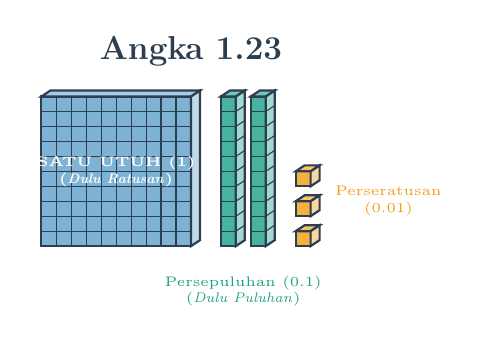
\begin{tikzpicture}[scale=0.38, baseline={([yshift=-.5ex]current bounding box.center)}]
        % The Whole (1)
        \DrawFlat{0}{0}
        % CHANGED COLOR TO WHITE FOR CONTRAST
        \node[font=\bfseries\tiny, text=white, align=center] at (2.5, 2.5) {SATU UTUH (1)\\(\textit{Dulu Ratusan})};
        
        % The Tenths (0.1)
        \DrawLong{6}{0} \DrawLong{7}{0}
        \node[font=\tiny, text=accentTeal, align=center] at (6.75, -1.5) {Persepuluhan (0.1)\\(\textit{Dulu Puluhan})};
        
        % The Hundredths (0.01)
        \DrawUnit{8.5}{0} \DrawUnit{8.5}{1} \DrawUnit{8.5}{2}
        
        % MOVED LABEL TO THE RIGHT (avoid overlap)
        \node[font=\tiny, text=niceOrange, align=center, anchor=west] at (9.5, 1.5) {Perseratusan\\(0.01)};
        
        \node[font=\bfseries\large, mainBlue] at (5, 6.5) {Angka 1.23};
    \end{tikzpicture}
\end{minipage}%
\hfill
\begin{minipage}{0.52\textwidth}
    \textbf{Konsep:} "Relativitas Unit".
    Siswa sering bingung desimal karena menganggap kubus kecil *selalu* 1. 
    Ubah definisi: "Jika Keping Besar ini adalah 1 Kue Utuh, maka 1 Batang adalah potongannya (0.1), dan Kubus Kecil adalah remahannya (0.01)."
\end{minipage}
\end{CaseStudyBox}

\vspace{0.3cm}

% --- KASUS 7 (ADDED) ---
\begin{CaseStudyBox}{KASUS 7: TRANSISI ALJABAR $(x+2)(x+1)$}
\begin{minipage}{0.45\textwidth}
    \centering
    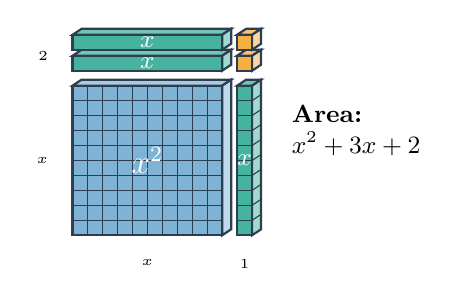
\begin{tikzpicture}[scale=0.38, baseline={([yshift=-.5ex]current bounding box.center)}]
        % x^2 (Flat)
        \DrawFlat{0}{0}
        \node[font=\bfseries\large, text=white] at (2.5, 2.5) {$x^2$};
        
        % x terms (Vertical Longs)
        \DrawLong{5.5}{0}
        \node[font=\bfseries\small, text=white] at (5.75, 2.5) {$x$};
        
        % x terms (Horizontal Longs - simulated by rotating dimensions manually)
        % Using DrawLong logic but rotated 90 degrees visually
        \begin{scope}[shift={(0,5.5)}]
             \draw[fill=accentTeal!80, draw=mainBlue, thick] (0,0) rectangle (5, 0.5);
             \draw[fill=accentTeal!60, draw=mainBlue, thick] (0,0.5) -- (0.3, 0.7) -- (5.3, 0.7) -- (5, 0.5) -- cycle;
             \draw[fill=accentTeal!40, draw=mainBlue, thick] (5,0) -- (5.3, 0.2) -- (5.3, 0.7) -- (5, 0.5) -- cycle;
             \node[font=\bfseries\small, text=white] at (2.5, 0.25) {$x$};
        \end{scope}
        \begin{scope}[shift={(0,6.2)}]
             \draw[fill=accentTeal!80, draw=mainBlue, thick] (0,0) rectangle (5, 0.5);
             \draw[fill=accentTeal!60, draw=mainBlue, thick] (0,0.5) -- (0.3, 0.7) -- (5.3, 0.7) -- (5, 0.5) -- cycle;
             \draw[fill=accentTeal!40, draw=mainBlue, thick] (5,0) -- (5.3, 0.2) -- (5.3, 0.7) -- (5, 0.5) -- cycle;
             \node[font=\bfseries\small, text=white] at (2.5, 0.25) {$x$};
        \end{scope}
        
        % Unit terms (1) filling the corner
        \DrawUnit{5.5}{5.5}
        \DrawUnit{5.5}{6.2}
        
        % Labels
        \node[left, font=\bfseries\tiny] at (-0.5, 2.5) {$x$};
        \node[left, font=\bfseries\tiny] at (-0.5, 6) {$2$};
        \node[below, font=\bfseries\tiny] at (2.5, -0.5) {$x$};
        \node[below, font=\bfseries\tiny] at (5.75, -0.5) {$1$};
        
        \node[align=left, font=\bfseries\small, anchor=west] at (7, 3.5) {Area:\\$x^2 + 3x + 2$};
    \end{tikzpicture}
\end{minipage}%
\hfill
\begin{minipage}{0.52\textwidth}
    \textbf{Konsep:} "Aljabar Geometris".
    Blok Dienes bukan hanya untuk aritmatika.
    Gunakan "Flat" sebagai $x^2$ (ukuran tak tentu), "Long" sebagai $x$, dan "Unit" sebagai 1.
    Ini membuktikan secara visual bahwa $(x+2)(x+1) = x^2 + 3x + 2$.
\end{minipage}
\end{CaseStudyBox}

\end{document}
